{\color{indiagreen}\subsection{Nastavitve}}
Kot smo že omenili v uvodu je Unity večplatformsko razvijalno orodje. Z Unity-jem lahko razvijamo aplikacije za:
\begin{itemize}
	\item Web Player
	\item Windows
	\item Mac OS X
	\item Linux
	\item IOS
	\item Android
	\item Tizen
	\item Windows Store
	\item Windows Phone 8
	\item WebGL
	\item Samsung TV
	\item BlackBerry
	\item Xbox 360
	\item Xbox One
	\item PS3
	\item PS Vita
	\item PS4
\end{itemize}
Seveda za nekatere platforme potrebujemo posebne licence ali Unity PRO verzijo ter seveda za posamezne platforme posebne SDK knjižnice.\\
Do vseh te nastavitev pa dostopamo tako, da odpremo \textbf{File} $\rightarrow$ \textbf{Build Settings...}. Nato se nam pojavi to okno:\\
\begin{figure}[ht!]
	\centering
	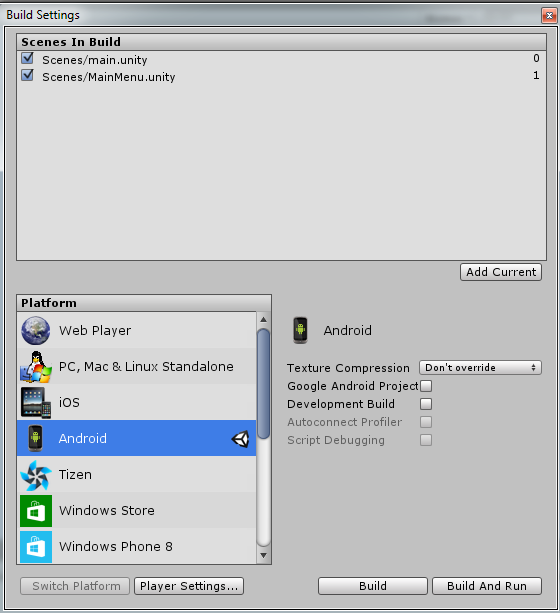
\includegraphics[width=8cm, height=8cm,keepaspectratio=true]{Building1.png}
	\caption{Build settings}
	{\tiny Vir: Osebni arhiv}
\end{figure}
Na sredini nam pokaže imena scen, ki se bojo zgradila v tej verziji. Imamo možnost, da dodamo trenutno sceno ali pa povlečemo sceno iz mape. Z lahkoto pa tudi odstranimo sceno tako, da jo odznačimo. Na levi strani vidimo katere platforme so nam na voljo. Levo spodaj je gumb \textbf{Switch Platform}, ki zamenja platformo za katero hočemo buildati. Zraven je gumb \textbf{Player Settings...}, ki po samem imenu malce zavaja. V bistvu nam odpre novo okno, kjer lahko za vsako platformo specificiramo na kakšen način se bo zgradila aplikacija. Imamo različne nastavitve od imena aplikacije, izbira ikone, resolucije, renderinga in tudi optimizacije. Več o tem bo povedal v naslednjem poglavju, ko se bom tudi osredotočil samo na android platformo.\\
\begin{figure}[ht!]
	\centering
	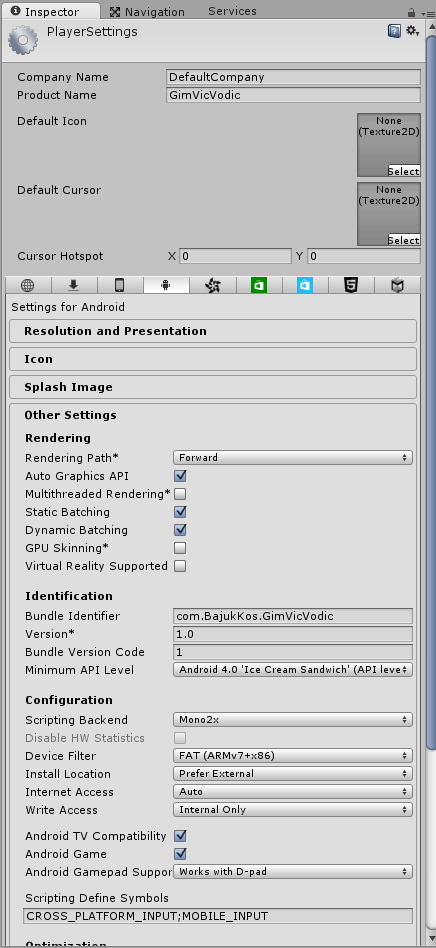
\includegraphics[width=8cm, height=8cm,keepaspectratio=true]{Building2.png}
	\caption{Player settings}
	{\tiny Vir: Osebni arhiv}
\end{figure}
Ostaneta nam samo še dva gumba, ki pa naredita točno to kar piše na njih. To sta \textbf{Build}, ki zgradi aplikacijo(naredi npr. .exe ali .apk datoteko) in \textbf{Build and Run}, ki jo še požene. In če izbrana platforma računalnik potem se zažene na računalniku, če gre za mobilno platformo, pa mora biti na računalnik povezan telefon in na računalniku mora biti SDK knjižnica, ko so izpolnjene vse te specifikacije se na telefonu namesti apk od aplikacije in se tudi požene.\\
Kateri koli gumb od teh nam vrne lahko datoteko z .apk, .exe ali katero drugo končnico v kateri je potem naša igra, ki jo lahko igramo, delimo z prijatelji in pokažemo staršem.